\section{Base Teórica}

La planificación es un componente esencial de cualquier sistema operativo, encargado de asignar tiempo de procesamiento a los diferentes hilos y procesos en ejecución. En este capítulo, nos sumergiremos en la comprensión de la planificación a corto plazo, con especial atención en el contexto del sistema operativo FreeBSD y su planificador 4BSD. Como ya se detalló previamente en el capítulo 1, este trabajo se basa y extiende directamente desde investigaciones previas\cite{bib1}, donde se introdujo el concepto de Redes de Petri, para el modelado de procesos.\par

Exploraremos los conceptos fundamentales de procesos e hilos, detallando su estructura, estados y dinámicas de ejecución. Además, nos adentraremos en el funcionamiento interno del planificador, desglosando las operaciones esenciales como el cambio de contexto, el encolado de procesos, la selección de procesador y la remoción de hilos de la cola. Estos aspectos son esenciales para comprender cómo el planificador 4BSD toma decisiones en tiempo real sobre la ejecución de procesos y la administración de recursos.\par

Al profundizar en esta base teórica, no solo sentaremos las bases para entender el funcionamiento del planificador de FreeBSD, sino que también estableceremos una sólida conexión con los avances y las decisiones tomadas en trabajos anteriores. Esto nos permitirá visualizar el progreso continuo y las oportunidades de mejora que surgieron a partir de esos primeros cambios implementados en el sistema operativo.\par

\subsection{Procesos e hilos}

En sistemas operativos, los procesos son entidades aisladas que representan la ejecución de una tarea o aplicación en particular. Cada proceso cuenta con su propio espacio de direcciones, que es un área reservada de memoria virtual donde se aloja el código del programa, las variables y los recursos necesarios para su ejecución. Además, disponen de acceso a los recursos del kernel a través de llamadas a sistemas.\par

Dentro de cada proceso, puede haber uno o varios hilos de ejecución. Estos hilos son unidades de ejecución independientes que comparten los recursos del proceso padre. Cada hilo se asocia con un procesador virtual, que tiene su propio contexto y un stack de ejecución alojado en el espacio de direcciones del proceso.\par

El kernel del sistema operativo crea la ilusión de ejecución concurrente de múltiples procesos, distribuyendo los recursos del sistema entre los procesadores listos para ejecutar tareas.\par

\subsubsection{Estructura de los procesos}
Cada proceso en el sistema recibe un identificador único llamado \textit{identificador de proceso} (PID). Los PID son el mecanismo común utilizado por las aplicaciones y el kernel para hacer referencia a los procesos. Existen dos identificadores que son de especial importancia para cada proceso: el PID del proceso en sí, y el PID del proceso padre.

La estructura simplificada de un proceso se puede observar en la Figura \ref{fig:process-state}. Esta estructura tiene como objetivo facilitar la gestión de múltiples hilos que comparten un espacio de direcciones y otros recursos dentro del proceso. Algunas de las categorías que componen esta estructura son las siguientes:

\begin{itemize}
    \item Identificación del grupo de procesos: el grupo de procesos y la sesión a la que pertenece el mismo son elementos importantes para la gestión y el control de los procesos en el sistema.
    \item Credenciales de usuario: los identificadores de usuario y grupo determinan los permisos de acceso a los recursos del sistema.
    \item Gestión de memoria: esta parte de la estructura es crucial para asignar y gestionar el espacio de direcciones virtuales del proceso, así como para administrar otros aspectos relacionados con la memoria.
    \item Descriptores de archivos: una matriz de punteros que indica los archivos abiertos por el proceso e información relevante de los mismos.
    \item Vector de llamadas al sistema: estructura de datos que mapea las llamadas al sistema con las funciones correspondientes en el kernel del sistema operativo.
    \item Contabilidad de recursos: estructura que describe la utilización de los recursos del sistema por parte del proceso.
    \item Estadísticas: estadísticas del proceso sobre su ejecución, temporizadores y profiling.
    \item Acciones de señal: la acción a tomar cuando se envía una señal a un proceso.
    \item Estructura de hilo: el contenido de la estructura de hilos del proceso.
\end{itemize}

\begin{figure}[H]
    \centering
    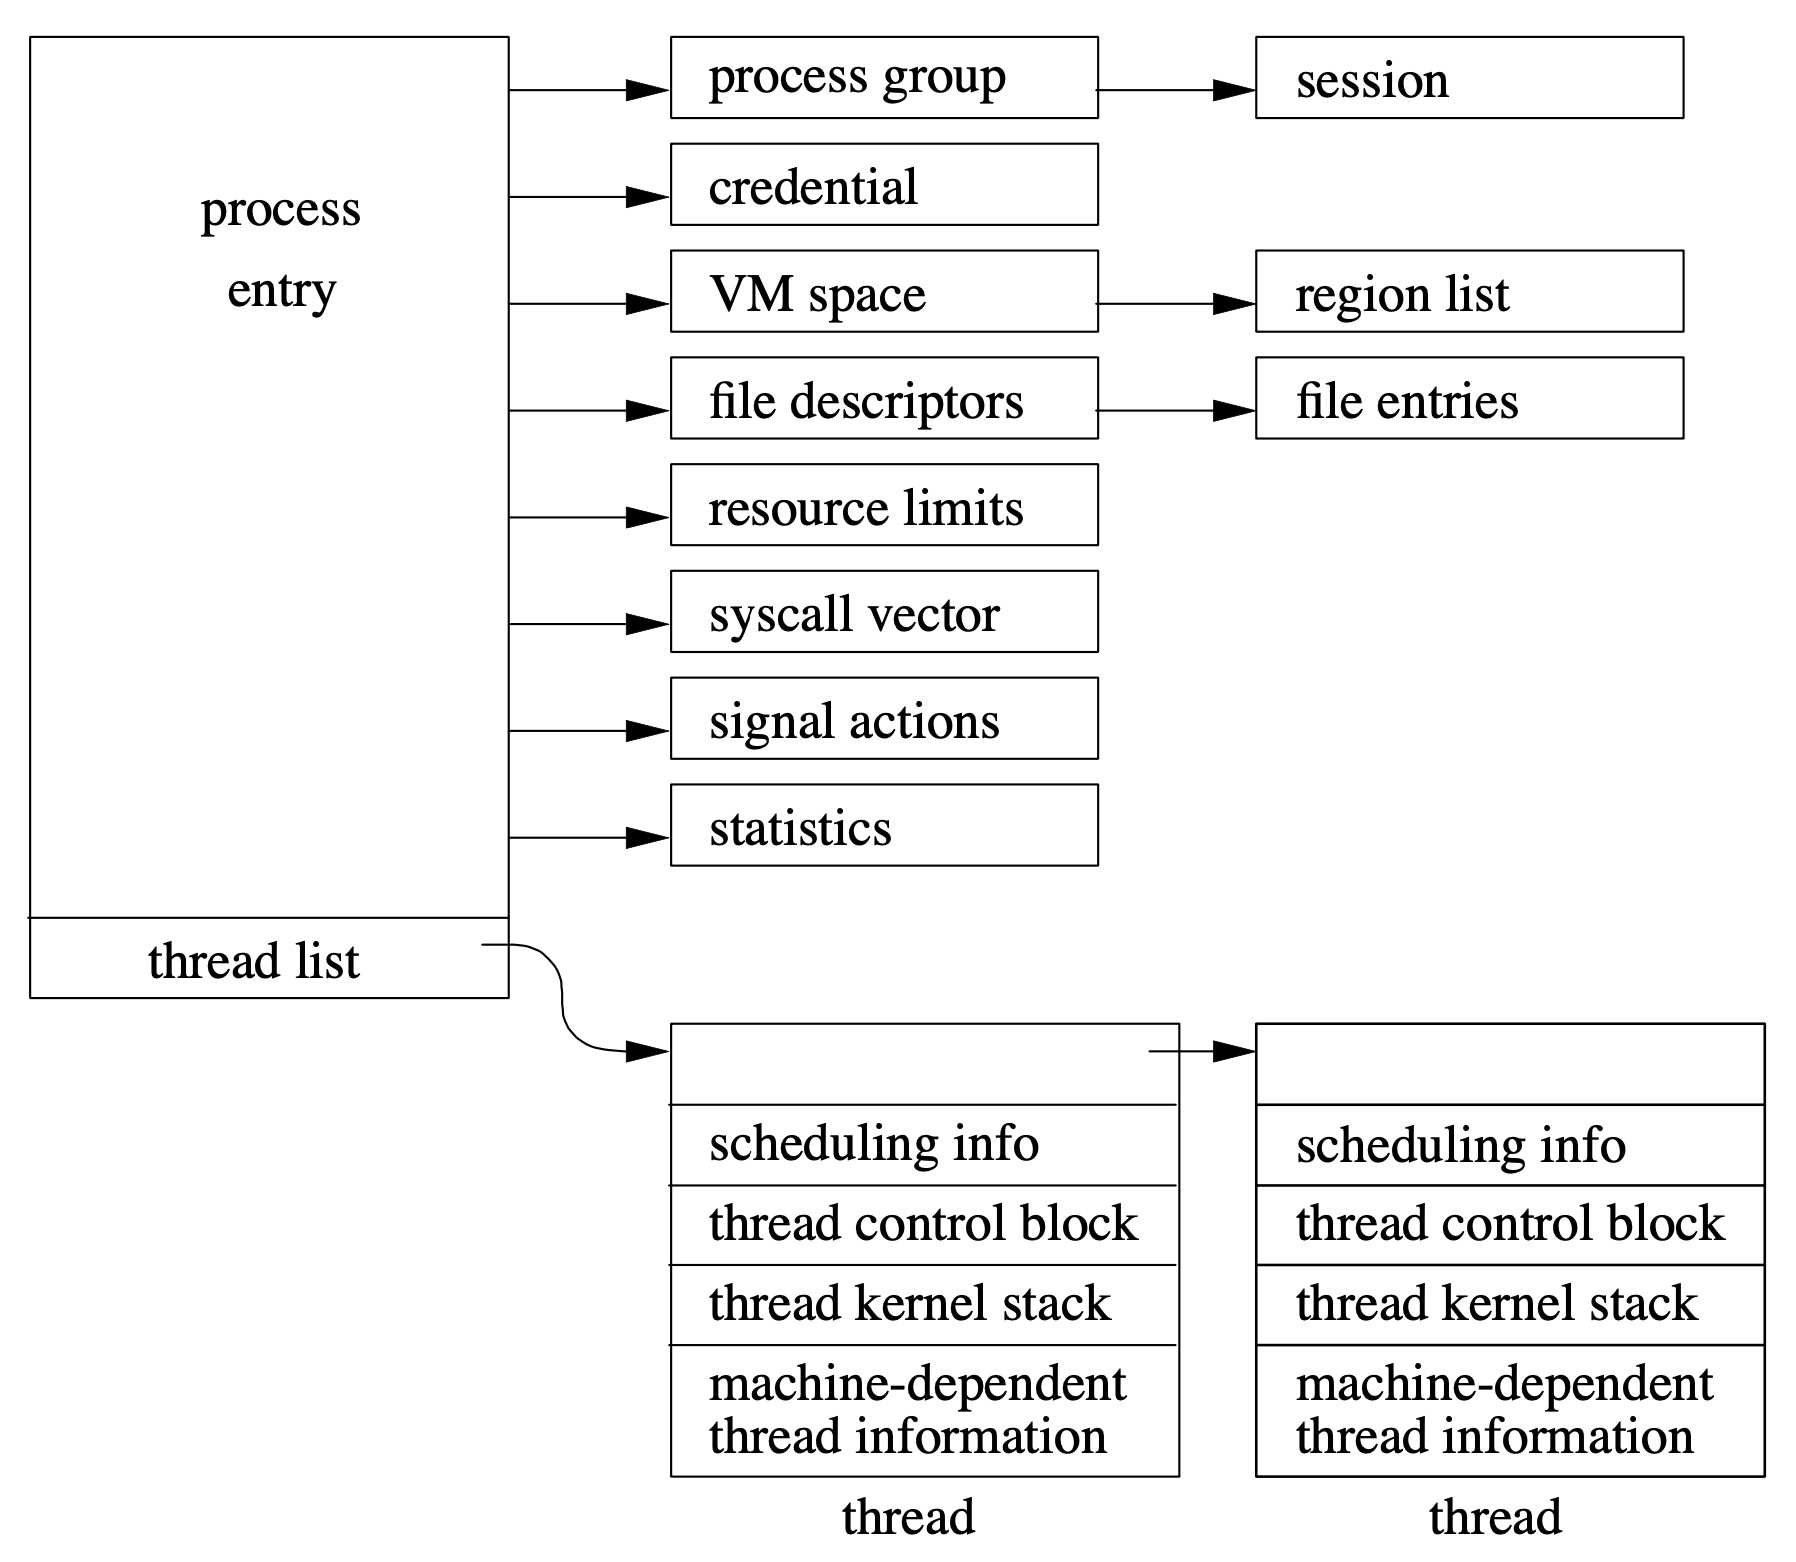
\includegraphics[width=0.5\textwidth]{./images/processStructure.png}
    \caption{Estructura simplificada de un proceso.}
    \label{fig:process-state}
\end{figure}

Cada proceso cuenta con los punteros \textit{p\_pptr}, \textit{p\_children} y \textit{p\_sibling}, utilizados para establecer la relacion entre procesos. Cuando se crea un proceso hijo, se agrega a la lista \textit{p\_children} de su padre. El proceso hijo también mantiene un enlace a su padre mediante su puntero \textit{p\_pptr}. Si un proceso tiene más de un hijo activo al mismo tiempo, los hijos están asociados entre sí a través de las entradas de la lista \textit{p\_sibling}. La Figura \ref{fig:process-hierarchy} muestra un ejemplo de jerarquia de procesos.

\begin{figure}[H]
    \centering
    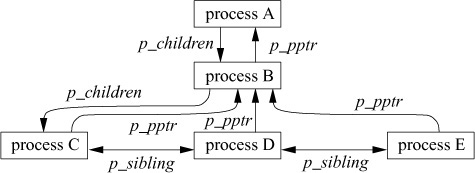
\includegraphics[width=0.5\textwidth]{./images/process-hierarchy.jpeg}
    \caption{Jerarquía de grupo de procesos.}
    \label{fig:process-hierarchy}
\end{figure}


\subsubsection{Estructura de los hilos}
Un hilo, en sistemas operativos modernos, constituye una unidad fundamental de ejecución dentro de un proceso. Se trata de una entidad independiente que representa una secuencia de instrucciones ejecutables dentro del contexto de un proceso. Cada hilo posee su propio contador de programa, registros de CPU y pila de ejecución, lo que le permite ejecutar código de manera concurrente dentro del mismo proceso. Aunque los hilos comparten recursos como el espacio de direcciones y otros recursos del proceso principal, también pueden comunicarse y cooperar entre sí para llevar a cabo tareas específicas de manera más eficiente.\par

En el caso de FreeBSD, el sistema adopta el modelo 1:1, donde cada hilo de usuario se corresponde con un hilo a nivel de kernel para mejorar la eficiencia de las aplicaciones.\par

La estructura de un hilo, que se muestra en la Figura \ref{fig:process-state}, contiene la información necesaria para ejecutarse en el kernel del sistema operativo:

\begin{itemize}
    \item Información para la planificación: se refiere a la prioridad del hilo en modo kernel y en modo usuario, la cantidad de tiempo que ha pasado suspendido y el uso reciente de la CPU. Además, se indica el estado de ejecución del hilo, banderas de estado adicionales; y si el hilo se encuentra suspendido, información sobre el canal y evento por el cual espera.
    \item TSB (thread state block): estado de ejecución del hilo en modo usuario y modo kernel. La estructura incluye registros de propósito general, punteros de pila, contador de programa, registros de gestión de memoria, entre otros.
    \item Pila del kernel: pila para usar al ejecutar en el kernel. Las pilas del kernel deben mantenerse pequeñas para evitar desperdiciar memoria física.
    \item Estado de la máquina (\textit{machine-dependent state}): se refiere a la información del hilo en relación a detalles que son específicos de la arquitectura de la CPU (registros de estado de punto flotante, información de interrupciones, información de registros de segmento de memoria, etc.).
\end{itemize}

\subsubsection{Estados de los procesos e hilos}

La estructura de un proceso en FreeBSD incluye un campo que indica su estado actual. Los estados de un proceso son fundamentales para entender su comportamiento en el sistema y están estrechamente relacionados con el funcionamiento del planificador 4BSD. Cuando se crea un proceso utilizando la llamada al sistema \textit{fork}, inicialmente se marca como nuevo (NEW). Este estado indica que el proceso está en su fase de creación y aún no ha recibido suficientes recursos para comenzar la ejecución.

Una vez que se asignan los recursos necesarios, el estado del proceso se cambia a NORMAL. En este estado, los hilos del proceso pueden encontrarse en diferentes subestados: ejecutable (RUNNABLE) cuando están listos para ejecutarse o actualmente en ejecución, durmiendo (SLEEPING) cuando están esperando un evento, o detenidos (STOPPED) cuando han sido pausados por una señal o por el proceso padre. El estado NORMAL persiste hasta que el proceso completa su tarea.

Cuando un proceso ha finalizado su ejecución, entra en el estado ZOMBIE. En este estado, el proceso ha liberado sus recursos pero aún no ha notificado formalmente su terminación al proceso padre. Es responsabilidad del sistema operativo limpiar los procesos en estado ZOMBIE y comunicar al proceso padre que el hijo ha finalizado.

La relación entre estos estados y el planificador 4BSD es crucial para comprender cómo se gestionan los recursos del sistema y cómo se asigna el tiempo de CPU a los procesos en FreeBSD.

En la tabla \ref{tabla:estados-proceso}, se proporciona una descripción concisa de cada estado del proceso y su significado en el contexto del sistema operativo.

\begin{table}[H]
    \centering
    \begin{tabular}{|c|l|}
        \hline
        \textbf{Estado} & \textbf{Características} \\
        \hline
        NEW & En fase de creación, aún sin recursos asignados \\
        \hline
        NORMAL & Ejecución activa, sus hilos alternaran entre \textit{RUNNABLE}, \textit{SLEEPING} o \textit{STOPPED} \\
        \hline
        ZOMBIE & En fase de finalización \\
        \hline
    \end{tabular}
    \caption{Descripción de los estados del proceso en FreeBSD}
    \label{tabla:estados-proceso}
\end{table}

En FreeBSD, el sistema organiza las estructuras de procesos en dos listas principales: \textit{zombproc} y \textit{allproc}. Los procesos en estado ZOMBIE se encuentran en la lista \textit{zombproc}, mientras que los procesos activos están en la lista \textit{allproc}. Esta distinción permite optimizar las operaciones del sistema, como la llamada al sistema \textit{wait} que busca procesos terminados, así como las operaciones del planificador que identifican procesos listos para ejecutarse.

Los hilos de un proceso, por su lado, excluyendo los que están en ejecución, se distribuyen en tres colas principales: \textit{run\_queue}, \textit{sleep\_queue} y \textit{turnstile\_queue}. Los hilos listos para ejecutarse se ubican en la \textit{run\_queue}, mientras que aquellos que están bloqueados esperando eventos se encuentran en la \textit{sleep\_queue} o en la \textit{turnstile\_queue}. Es importante destacar que las colas \textit{run\_queue} están organizadas según la prioridad de planificación de hilos establecida por el planificador 4BSD. La diferencia entre la \textit{turnstile\_queue} y la \textit{sleep\_queue}, radica en que esta última se utiliza para hilos bloqueados con locks de tipo \textit{sleepable}, mientras que la \textit{turnstile\_queue} alberga hilos bloqueados con locks de tipo \textit{non-sleepable}.

\subsubsection{Prioridad de los hilos}

Las prioridades de los hilos son un componente importante para la planificación. Estas prioridades, que van desde 0 hasta 255 (donde 0 denota la prioridad más alta), determinarán el orden en que se ejecutarán los hilos. En la Tabla \ref{tabla:prio-hilos}, se describen los diferentes rangos de prioridades.

Las prioridades en el rango de 0 a 47 son asignadas de forma predeterminada por el sistema y se destinan a las tareas de interrupción.\par

Las prioridades de los hilos en tiempo real se encuentran en el intervalo de 48 a 79 y deben ser configuradas previamente por las aplicaciones mediante la llamada al sistema \textit{rtprio}. A continuación, se encuentran los hilos con prioridades en el rango de 80 a 119, conocidos como hilos del kernel superior (top-half kernel threads). Estos hilos se encargan de gestionar operaciones críticas del kernel que afectan a todo el sistema.\par

Los hilos con prioridades entre 120 y 223 pertenecen a la clase de hilos de tiempo compartido. Están destinados a ejecutar tareas de usuario convencionales y sus prioridades son ajustadas de manera automática por el kernel en función del uso de la CPU.\par

Cuando no hay tareas activas que requieran el uso de la CPU, los hilos de la clase \"IDLE\" pueden ejecutarse. Estos hilos tienen la finalidad de mantener el sistema en un estado inactivo, consumiendo recursos mínimos y estando listos para responder a tareas prioritarias.\par

\begin{table}[H]
    \centering
    \begin{tabular}{|c|c|c|}
        \hline
        \textbf{Rango} & \textbf{Clase} & \textbf{Tipo de hilo} \\
        \hline
        0 - 47 & ITHD & Bottom-half kernel (interrupt) \\
        \hline
        48 -79 & REALTIME & Real-time user \\
        \hline
        80 - 119 & KERN & Top-half kernel \\
        \hline
        120 - 223 & TIMESHARE & Time-sharing user \\
        \hline
        224 - 255 & IDLE & Idle user \\
        \hline
    \end{tabular}
    \caption{Clases de hilos por rango de prioridad.}
    \label{tabla:prio-hilos}
\end{table}


\subsection{Planificación}

La planificación en sistemas operativos, implica decidir el orden y la duración de la ejecución de procesos e hilos del sistema. En este sentido, es el componente clave para optimizar el uso de recursos y el tiempo de ejecución de los programas.\par

FreeBSD cuenta con el planificador 4BSD, un planificador de tiempo compartido (\textit{timeshare scheduler}) que asigna dinámicamente la prioridad de los procesos. Este cálculo se realiza en función de varios parámetros, como la cantidad de tiempo de CPU utilizado, la cantidad de recursos de memoria que posee o requiere para su ejecución, entre otros.\par

La política de planificación asigna inicialmente una prioridad de ejecución alta a cada hilo y permite que ese hilo se ejecute durante un intervalo de tiempo fijo, o \textit{time slice}. A los hilos que se ejecutan durante la duración de su \textit{time slice} se les decrementa la prioridad; mientras que los hilos que ceden la CPU (generalmente debido a operaciones de entrada/salida) pueden mantener su prioridad. Por otro lado, los hilos inactivos incrementan su prioridad.\par

Esta forma de planificación beneficia especialmente a los programas interactivos. Los procesos que demandan una gran cantidad de tiempo de CPU ven reducida rápidamente su prioridad, mientras que los procesos interactivos que permanecen mayormente inactivos conservan una prioridad elevada. Esto permite que, cuando estén listos para ejecutarse, puedan desplazar a los procesos de baja prioridad que llevan ejecutándose durante un largo periodo de tiempo. Por ejemplo, supongamos que un editor de texto realiza una búsqueda dentro del documento, lo que conlleva un aumento temporal en el uso de recursos computacionales. Durante este período, la prioridad del editor puede verse momentáneamente reducida para dar prioridad a otros procesos más urgentes. Sin embargo, una vez completada la búsqueda y sin actividad adicional del usuario, el editor recuperará su prioridad en la cola de planificación del sistema operativo.\par

Algunas tareas requieren un control más preciso sobre el proceso, como el caso de la planificación de tiempo real. FreeBSD también implementa esta funcionalidad mediante una cola separada para los hilos en cuestión, los cuales no se ven interrumpidos por otros hilos a menos que tengan igual o mayor prioridad. Además, el \textit{kernel} de FreeBSD cuenta con otra cola de hilos de mínima prioridad que se ejecutan únicamente cuando ningún hilo en las colas de mayor prioridad está en un estado de posible ejecución.\par

\subsubsection{Multilevel Feedback Queue Scheduling}
% https://www.geeksforgeeks.org/multilevel-feedback-queue-scheduling-mlfq-cpu-scheduling/

% Pag 120 del PDF de 4.4BSD (no el de freebsd)

% multilevel feedback queue: A queueing scheme in which requests are partitioned into multiple prioritized subqueues, with requests moving between subqueues based on dynamically varying criteria. The 4.4BSD kernel uses a multilevel- feedback-queueing scheme for scheduling the execution of processes.


\subsection{Conceptos del proyecto integrador previo}

% El scheduler se encarga de planificar aquellos hilos correspondientes a procesos en estado NORMAL. Los hilos que conforman un proceso pueden encontrarse en diferentes estados:

% \begin{itemize}
%     \item \uppercase{inactive}: En proceso de creación y aún no han sido inicializados.
%     \item \uppercase{inhibited}: Esperando por algún recurso del sistema o evento antes de poder ejecutarse.
%     \item \uppercase{can\_run}: Inicializados y disponibles para ser agregados a alguna cola de ejecución.
%     \item \uppercase{runq}: En la cola de ejecución, esperando su turno para ser ejecutados.
%     \item \uppercase{running}: En ejecución.
% \end{itemize}

\subsubsection{Introducción}

El proyecto integrador del cual partimos, consiste en modelar el planificador 4BSD con Redes de Petri. Los hilos de ejecución de un proceso como el planificador del sistema operativo pueden considerarse como sistemas que pueden modelarse utilizando esta herramienta.\par

Las decisiones de encolado de los hilos en una CPU se toman a partir de la información representada en el modelo; así como también los estados globales y los de cada hilo.\par

% TODO{TODO: Agregar un poco mas para mejorar}

\subsubsection{Elección del planificador}

La planificación a corto plazo en FreeBSD ha experimentado una evolución constante desde sus primeras versiones basadas en el sistema operativo 4.4BSD\cite{bib3}. A lo largo de su historia, FreeBSD ha confiado en dos planificadores para gestionar la asignación de recursos del sistema, siendo el planificador 4BSD uno de los más notables. Este planificador, inicialmente diseñado para sistemas monoprocesador, ha sido adaptado y optimizado para entornos multiprocesador, convirtiéndose en un componente fundamental de la arquitectura del sistema operativo.\par

Aunque el planificador 4BSD es más simple en comparación con los más modernos, ha demostrado ser rápido y eficiente para satisfacer las necesidades de muchos usuarios. Sin embargo, con el objetivo de mejorar aún más el rendimiento y la capacidad de respuesta del sistema, se introdujo el planificador ULE en la versión 5.0 de FreeBSD. El ULE ofrece características avanzadas que lo hacen más adecuado para entornos con cargas de trabajo más complejas y exigentes.\par

A pesar de que el planificador ULE se ha convertido en el predeterminado en las versiones más recientes de FreeBSD (a partir de la versión 8.0), el planificador 4BSD sigue siendo una opción estable y confiable. La comunidad de FreeBSD continúa manteniendo y brindando soporte para el planificador 4BSD, asegurando su disponibilidad para aquellos que prefieren su simplicidad y eficiencia. Además, no hay planes inmediatos por parte del equipo de desarrollo de FreeBSD para dejar de darle soporte.\par

Nuestro proyecto se basa en el trabajo previo realizado en el marco del proyecto integrador, que se centró en el planificador 4BSD. Para obtener una comprensión más detallada y contextualizada de esta elección, se puede consultar las secciones de \textit{Alcance} (1.4) y  \textit{Diferencias entre el planificador ULE y el 4BSD} (2.3.3) del proyecto integrador previo\cite{bib1}. Aunque nuestro enfoque principal no radica en realizar cambios inmediatos en el sistema operativo ni en contribuir directamente a la comunidad de FreeBSD, continuamos con la fase de investigación e implementación centrada en este tipo de planificadores.\par


--- PLANIFICADOR

\subsubsection{Funcionamiento del planificador 4BSD}

El planificador 4BSD, inicialmente diseñado para sistemas monoprocesador, ha evolucionado para adaptarse eficazmente a sistemas multiprocesador. Comprender su funcionamiento es esencial para apreciar cómo este componente crítico del sistema FreeBSD gestiona la asignación de recursos y el tiempo de ejecución de los hilos.\par

En esencia, el planificador 4BSD organiza los hilos en múltiples colas según su prioridad. Cada hilo tiene una prioridad asignada y reside en una cola específica de acuerdo con esta prioridad.\par

Un aspecto crucial del planificador 4BSD es la gestión de tiempos de ejecución equitativos. A cada proceso se le asigna un pequeño período de tiempo, conocido como "timeslice". Una vez que un proceso agota su timeslice, se suspende temporalmente para permitir que otros procesos tengan la oportunidad de ejecutarse. Este proceso cíclico de asignación de tiempos de ejecución, basado en el algoritmo "Round Robin", asegura que ningún proceso monopolice los recursos del sistema durante largos períodos, contribuyendo así a un rendimiento estable y justo del sistema,  garantizando la equidad en el uso de los recursos del sistema.\par

En lo que respecta a las prioridades, el planificador 4BSD las ajusta periódicamente en función del tiempo de CPU consumido por cada hilo. Este proceso implica elevar la prioridad de los hilos que han utilizado menos tiempo de CPU y reducir la prioridad de aquellos que han consumido más recursos de procesador. De esta manera, el planificador se encarga de equilibrar la carga de trabajo de manera equitativa entre todos los procesos en ejecución en el sistema.\par


\subsubsection*{Funciones basicas del planificador}

intro en donde se explica que todas las funciones de aca abajo basicamente fueron las que tuvieron que cambiar para la planificacion con RdP

% TODO{Encolado (add)}
El sistema usa 64 colas, seleccionando una cola para un determinado hilo y dividiendo la prioridad del hilo por 4. Para ahorrar tiempo, los hilos en cada cola no se vuelven a dividir en prioridades.\par

Estas colas pueden ser de tipo run queue, turnstile queue o sleep queue. Los hilos en estado RUNNABLE se ubican en las colas de tipo run queue; mientras que los que están bloqueados o esperando un evento, son posicionados en los otros dos tipos de colas.\par

Si un hilo agota su tiempo (o intervalo de tiempo) permitido, se coloca al final de la cola de la que procede, y el próximo hilo (ahora al principio de la cola) se selecciona para ejecutarse.\par

Si un hilo se bloquea, no se vuelve a colocar en la cola de ejecución (run queue). En su lugar, se coloca en una turnstile queue o en una sleep queue.\par

Las operaciones relacionadas al encolado se realizan dentro de la función sched\_add(). Ésta función recibe como parámetros el hilo a encolar y flags con información acerca del mismo.\par

Su primera tarea es corroborar que el hilo se encuentre en un estado permitido para ser encolado, es decir, en estado CAN\_RUN o RUNNING. Al pasar esta verificación, se adquiere el lock del planificador y se lo pasa al estado RUNQ para luego elegir en cuál cola de CPU va a ser asignado. Esto es posible a través de la función sched\_pickcpu(), la cual elige un CPU de la siguiente forma:

\begin{enumerate}
    \item Consulta si el hilo ya se había ejecutado en un procesador anterior y si es posible volverlo a encolar en el mismo. En caso de que sea verdadero, almacena este valor en una variable. En caso contrario, dentro de esa variable guarda el valor NOCPU (igual a -1).
    \item Luego itera a través de cada CPU disponible en el sistema. En caso de que el CPU que se está iterando no permita el encolado, continúa con el siguiente.
    \item Para el caso en que esté permitido el encolado para el CPU que se está iterando, existen dos opciones basadas en el valor de la variable inicializada en el primer punto.
    \begin{enumerate}
        \item En caso de que la variable haya sido inicializada con el valor NOCPU, se la sobreescribe con el CPU de la iteración en la que se encuentra el programa en ese momento.
        \item En caso de que la variable haya sido inicializada con el valor del último CPU en el que había sido ejecutado el hilo, se consulta si la cola del CPU que se está iterando, tiene menor cantidad de procesos que la del CPU elegido en el punto 1. Caso afirmativo, se reemplaza el valor de la variable por el CPU que se está iterando, ya que esto significa que éste procesador contiene menos hilos en su cola de ejecución. Caso contrario, el valor de la variable no se sobreescribe.
    \end{enumerate}
    \item Al finalizar la iteración de cada CPU, se retorna el valor de la variable con el CPU más apropiado para el hilo.
\end{enumerate}

Una vez elegido el mejor CPU para el hilo, se procede a realizar los cambios de contexto necesarios para agregarlo a la cola del procesador correspondiente.

Si el procesador al que se agrega el hilo es diferente al que está ejecutando la función en ese instante, éste último envía una señal IPI (inter-processor interrupt) para comunicar que existe este nuevo hilo en su cola.

En caso de que el hilo se agregara a la cola del CPU actual, se llama a las funciones correspondientes para saber si este hilo tiene mayor prioridad que el que está en ejecución actualmente y debe reemplazarlo, esto se conoce como preemption.

% TODO{Cambios de contexto (switch y throw)}
Al hablar de cambios de contexto de los hilos, se hace referencia a dos funciones en particular.\par

La función sched\_switch() se encarga de expulsar al hilo que recibe por parámetro (hilo actual en ejecución), o en caso de que el hilo continúe en estado RUNNING por alguna razón, se vuelve a poner en cola a través de la función sched\_add().\par

Una vez finalizada la expulsión se solicita un nuevo hilo para ejecutar. Esto se hace a través de la función choosethread() y sched\_choose().\par

Una vez obtenido el nuevo hilo, se verifica que éste no sea el mismo que fue puesto en cola anteriormente, si esto sucediera, sólo continúa la ejecución. Pero en caso de que sean dos hilos diferentes, se procede a realizar el cambio de contexto haciendo uso de la función cpu\_switch().\par

La función cpu\_switch() guarda el contexto del hilo anterior y restaura el contexto del nuevo hilo. Así como también, se asegura de que el estado del nuevo hilo se marque como TD\_RUNNING (en ejecución).\par

Otra de las funciones que se encargan del cambio de contexto es sched\_throw(), la cual se encarga de cambiar un hilo por otro en el mismo CPU que se está ejecutando. Recibe un hilo como parámetro (el cual puede ser nulo), y lo expulsa del planificador. Luego a través de la misma función utilizada anteriormente, choosethread(), obtiene un nuevo hilo y continúa con su ejecución.\par

% TODO{Elección de hilos (choose)}
La elección del próximo hilo a ejecutar se hace a través de la función sched\_choose() previamente invocada por la función choosethread() nombrada anteriormente.

El funcionamiento consiste en elegir al hilo con mayor prioridad dentro de alguna de las colas no vacías del CPU o de la cola global. Cada hilo habilitado para ser ejecutado, es decir en estado RUNNABLE, tiene una prioridad asignada.

La función comienza obteniendo el primer hilo de la cola global y el primero de la cola del CPU; guardando ambos en dos variables diferentes. Luego compara las prioridades de ambos y se queda con el de mayor prioridad.

Una vez elegido el hilo, se procede a removerlo de la cola correspondiente, ya sea la global o la del CPU, y se retorna este hilo.

Para el caso en que ambos hilos sean nulos, es decir, no hay hilos para ejecutar, se simula una ejecución con el idlethread y se retorna el mismo.

% TODO{Remoción de hilos de la cola (rem)}
A diferencia de la función anterior, en la que al elegir un hilo para correr, éste era removido de la cola en la que estaba ubicado, la función sched\_rem() se utiliza para quitar un hilo (especificado por parámetro) de una cola por dos razones principales.\par

Una de estas es el ajuste de prioridad que consiste en otorgarle una nueva prioridad al hilo por lo que es necesario removerlo de la cola en la que se encuentra y luego volver a encolarlo a través de la función sched\_add() en la posición correspondiente.\par

El otro motivo por el cual se querría hacer uso de esta función es en caso de que un hilo tenga afinidad con algún CPU, por lo que el procedimiento será igual al mencionado en el párrafo anterior, con el objetivo de que se encuentre en la cola correcta.\par


----- RED DE PETRI

\subsubsection{Modelado del hilo}
Uno de los modelos representados a través de la Red de Petri, es el de los estados de un hilo. En la figura es posible observar esta representación.\par

% TODO{Agregar red de petri del hilo}

\begin{itemize}
    \item \textbf{T0\_INIT}: El paso del estado INACTIVE a CAN\_RUN. Esto sucede cuando el hilo se agrega al planificador. Esto sucede generalmente en el momento de creación de un proceso o cuando el mismo realiza un fork. Esta tarea no corresponde al scheduler, por lo que inicialmente un hilo en el planificador se encuentra inicializado en el estado CAN\_RUN. Esta transición nunca se dispara, solo se la incorpora al modelo de modo representativo.
    \item \textbf{T1\_ON\_QUEUE}: El hilo se pone en una cola local de una determinada CPU o en la cola global dependiendo de la disponibilidad. Esta cola organiza los hilos de acuerdo a sus prioridades de ejecución.
    \item \textbf{T2\_SET\_RUNNING}: El hilo se quita de la cola y pasa a ejecutar las instrucciones del programa que tiene asignadas. En este instante el procesador se encuentra ocupado por dicho hilo.
    \item \textbf{T3\_SWITCH\_OUT}: El scheduler interrumpe el hilo y lo vuelve a colocar en una cola. El planificador toma otro hilo de la cola (el de mayor prioridad) y realiza un cambio de contexto.
    \item \textbf{T4\_TO\_WAIT\_CHANNEL}: Algún evento, semáforo o espera bloquea al hilo. Se agrega en una sleep queue o turnstile, en la cual el hilo queda a la espera de un evento que le quitará el bloqueo.
    \item \textbf{T5\_WAKEUP}: Se desbloquea el hilo y puede volver a encolarse nuevamente. El evento que lo desbloquea se genera fuera del scheduler. El hilo queda a la espera para poder cambiar de estado cuando corresponda.
    \item \textbf{T6\_REMOVE}: Se ejecutará cada vez que un hilo deba ser expulsado de la cola en que se encuentra actualmente.
\end{itemize}


\subsubsection{Modelado del planificador}

Para modelar el planificador se hace un modelo específico para un procesador y se extiende para los demás. En este proyecto se consideran cuatro procesadores.

% TODO{Agregar red de petri de 1 procesador}

Transiciones
\begin{itemize}
    \item TRAN\_ADDTOQUEUE: Un hilo es agregado a la cola del CPU correspondiente. Se encuentra inhibida cuando todo el sistema se encuentra en modo monoprocesador (al inicio del sistema operativo); y cuando ya existe un hilo en la cola.
    \item TRAN\_UNQUEUE: Se quita al hilo próximo a ejecutar de la cola del CPU. En este punto el hilo se encuentra listo para ser ejecutado.
    \item TRAN\_EXEC: El hilo pasa a ejecución por lo que el recurso del procesador se encuentra ocupado. Esta transición elimina el token de la plaza de habilitación, permitiendo así que un nuevo hilo pueda ser encolado. A su vez, ésta transición se encuentra inhibida en el modo monoprocesador.
    \item TRAN\_EXEC\_EMPTY: Esta transición se comporta de igual manera que la anterior, pero no depende de la plaza de habilitación. Su utilidad surge para los hilos provenientes de la cola global.
    \item TRAN\_RETURN\_VOL: Representa un retorno del recurso procesador para que pueda ejecutar otro hilo de su cola. Más precisamente, se dispara cuando la interrupción de la ejecución se debe a que el hilo no puede continuar porque espera por un evento o un recurso.
    \item TRAN\_RETURN\_INVOL: El funcionamiento es igual a la transición anterior, pero en este caso se dispara cuando la interrupción se produce porque el hilo consumió su tiempo asignado de CPU o bien finalizó su tarea.
    \item TRAN\_FROM\_GLOBAL\_CPU: Representa el desencolado de un hilo desde la cola global.
    \item TRAN\_REMOVE\_QUEUE: Expulsa un hilo de la cola y también resta un token de habilitación de la CPU, es decir, se premia a la misma para que pueda encolar.
    \item TRAN\_REMOVE\_EMPTY\_QUEUE: Su funcionamiento es igual al anterior pero se ejecuta en los casos en que la plaza de habilitación no posea ningún token.
    \item TRAN\_REMOVE\_GLOBAL\_QUEUE: Expulsa un hilo de la cola global. No premia al CPU.
    \item TRAN\_START\_SMP: Se dispara cuando el sistema pasa de monoprocesador a multiprocesador.
    \item TRAN\_THROW: Se ejecutará automáticamente cada vez que todas las plazas de habilitación de las CPU tengan al menos un token. El objetivo de esta transición consiste en habilitar las colas con la menor cantidad de hilos que estaban inhibidas, una vez que todas se han emparejado.
    \item TRAN\_QUEUE\_GLOBAL: Agrega un hilo a la cola global.
\end{itemize}


\subsubsection{Jerarquía de transiciones}
Para llevar a cabo la conexión entre las redes de los hilos y la red de recursos de las CPU se utiliza el concepto de redes jerárquicas. Es decir que al dispararse cierta transición en la red de recursos, también debe dispararse su transición correspondiente en la red del hilo.

Las jerarquías están definidas de la siguiente forma:
\begin{itemize}
    \item Transiciones TRAN\_ADDTOQUEUE y TRAN\_QUEUE\_GLOBAL de la red de recursos son jerárquicas a la transición T1\_ON\_QUEUE del hilo.
    \item Transiciones TRAN\_EXEC y TRAN\_EXEC\_EMPTY de la red de recursos son jerárquicas a la transición T2\_SET\_RUNNING del hilo.
    \item Transiciones TRAN\_REMOVE\_QUEUE, TRAN\_REMOVE\_EMPTY\_QUEUE y TRAN\_ REMOVE\_GLOBAL\_QUEUE de la red de recursos son jerárquicas a la transición T6\_ REMOVE del hilo.
    \item Transición TRAN\_RETURN\_INVOL de la red de recursos es jerárquica a la transición T3\_ SWITCH\_OUT del hilo.
    \item Transición TRAN\_RETURN\_VOL de la red de recursos es jerárquica a la transición T4\_TO \_WAIT\_CHANNEL del hilo.
\end{itemize}

\subsubsection{Marcado inicial}
La red de recursos se inicializará siempre con un token en la plaza que indica que el sistema se encuentra funcionando en modo monoprocesador. Además, se inicializan las plazas que representan a las CPU con un token, excepto la de la CPU0 ya que la misma, inicialmente se encuentra ejecutando el hilo inicial del sistema, por lo que esta última debe inicializarse con un token en la plaza de ejecución (PLACE\_EXECUTING\_0).

